\documentclass[titlepage]{article}

\usepackage[english]{babel}
\usepackage{pdfpages} 
\usepackage{sidecap}
\usepackage{wrapfig}


%
\usepackage[top=1.5in, bottom=1.5in, left=2in, right=2in]{geometry}

\newcommand{\myparagraph}[1]{\paragraph{#1}\mbox{}\\}

\addtolength{\oddsidemargin}{-.875in}
\addtolength{\evensidemargin}{-.875in}
\addtolength{\textwidth}{1.75in}

\def \TACS {Track and Control System}

\begin{document}

\title{
\textbf{
Object Design Description}
\protect\\
for the
\protect\\
\textbf{
Track and Control System}
\protect\\
{\small Version 1.0}}

\author{Robert Moss, Aaron Periera, Matthew Shrago}
\maketitle

\newpage
\tableofcontents{} 
\newpage

\section{Introduction}

\subsection{Object Design Trade-offs}

\subsubsection{Buy vs. Build}
There is no product on the market that allows a user to control certain features around their Windows environment simply by tracking ones head. For this reason, we will have to build such a system, because buying it is not an option.
	

\subsubsection{Space vs. Speed}
In TACS, space is not a major priority. With only settings being kept, speed is the most crucial; as a fluid motion experience is what it is striving for. The latency at which the program registers the users movement will rely heavily on speed. The efficiency of the implementation will be directly related to the user experience (pertaining to speed).

\subsubsection{Delivery Time vs. Functionality}
If the development of TACS is behind schedule, certain tracking algorithms and windows features can be scrapped. The modularity of the design allows for this. Also, it's worth mentioning that TACS only needs one method of tracking, yet it's nice to give the user options.

\subsubsection{Delivery Time vs. Quality}
If testing runs behind schedule, the software can still be released and updates can be released to fix bugs at a later date. As long as the core functionality and at least one tracking module has been implemented, the product can be delivered.

\subsubsection{Files vs. Databases}
Files would not be as beneficial as a database because the data for TACS is not voluminous. A database would provide a sufficient structure to organize user settings. In using a file, users can theoretically edit and thus corrupt the file and the data inside. An "off site" database would be more secure and less likely to be modified.

\subsection{Interface Documentation Guidelines}
\textbf{\textit{Classes}, \textit{Interfaces} \& \textit{Packages}}: These names should be in \textit{Pascal Case}.
\begin{itemize}
	\item i.e.: ObjectTracker, TrackingModule, TrackingPackage
\end{itemize}
\textbf{\textit{Constants}}: All constants should be entirely in \textit{Upper Case}.
\begin{itemize}
	\item i.e.: RESOLUTION
\end{itemize}
\textbf{\textit{Identifiers} \& \textit{Methods}}: Identifier and Method names should be in \textit{Camel Case}.
\begin{itemize}
	\item i.e.: xPosition, yPosition, setWindow()
\end{itemize}
\textbf{\textit{Local Variables}}: Variables should be in all \textit{Lowercase}.
\begin{itemize}
	\item i.e.: speed
\end{itemize}

\subsection{Definitions, Acronyms, and Abbreviations}
\begin{itemize}
	\item Application Specific Definitions
	\begin{itemize}
		\item TACS - Track and Control System
		\item TM - Tracking Module
		\begin{itemize}
			\item OT - Object Tracker
			\item FRT - Facial Recognition Tracker
		\end{itemize}
		\item WCM - Windows Control Module
		\begin{itemize}
			\item WGO - Windows Grid Organizer
			\item WP - Windows Perspective
		\end{itemize}
		\item SM - Settings Module
	\end{itemize}
	\item Industry Definitions
	\begin{itemize}
		\item ODD - Object Design Description
		\item OpenCV - Open Computer Vision: An open source library for object tracking via the camera.
		\item SQLite - A lightweight, low maintenance, self contained local database.
		\item DB - Database
		\item RGB - Red, Green, Blue color values.
		\item HSV - Hue, Saturation, Value.
	\end{itemize}
\end{itemize}

\section{Packages}
\subsection{Package Diagram}
\begin{center}
	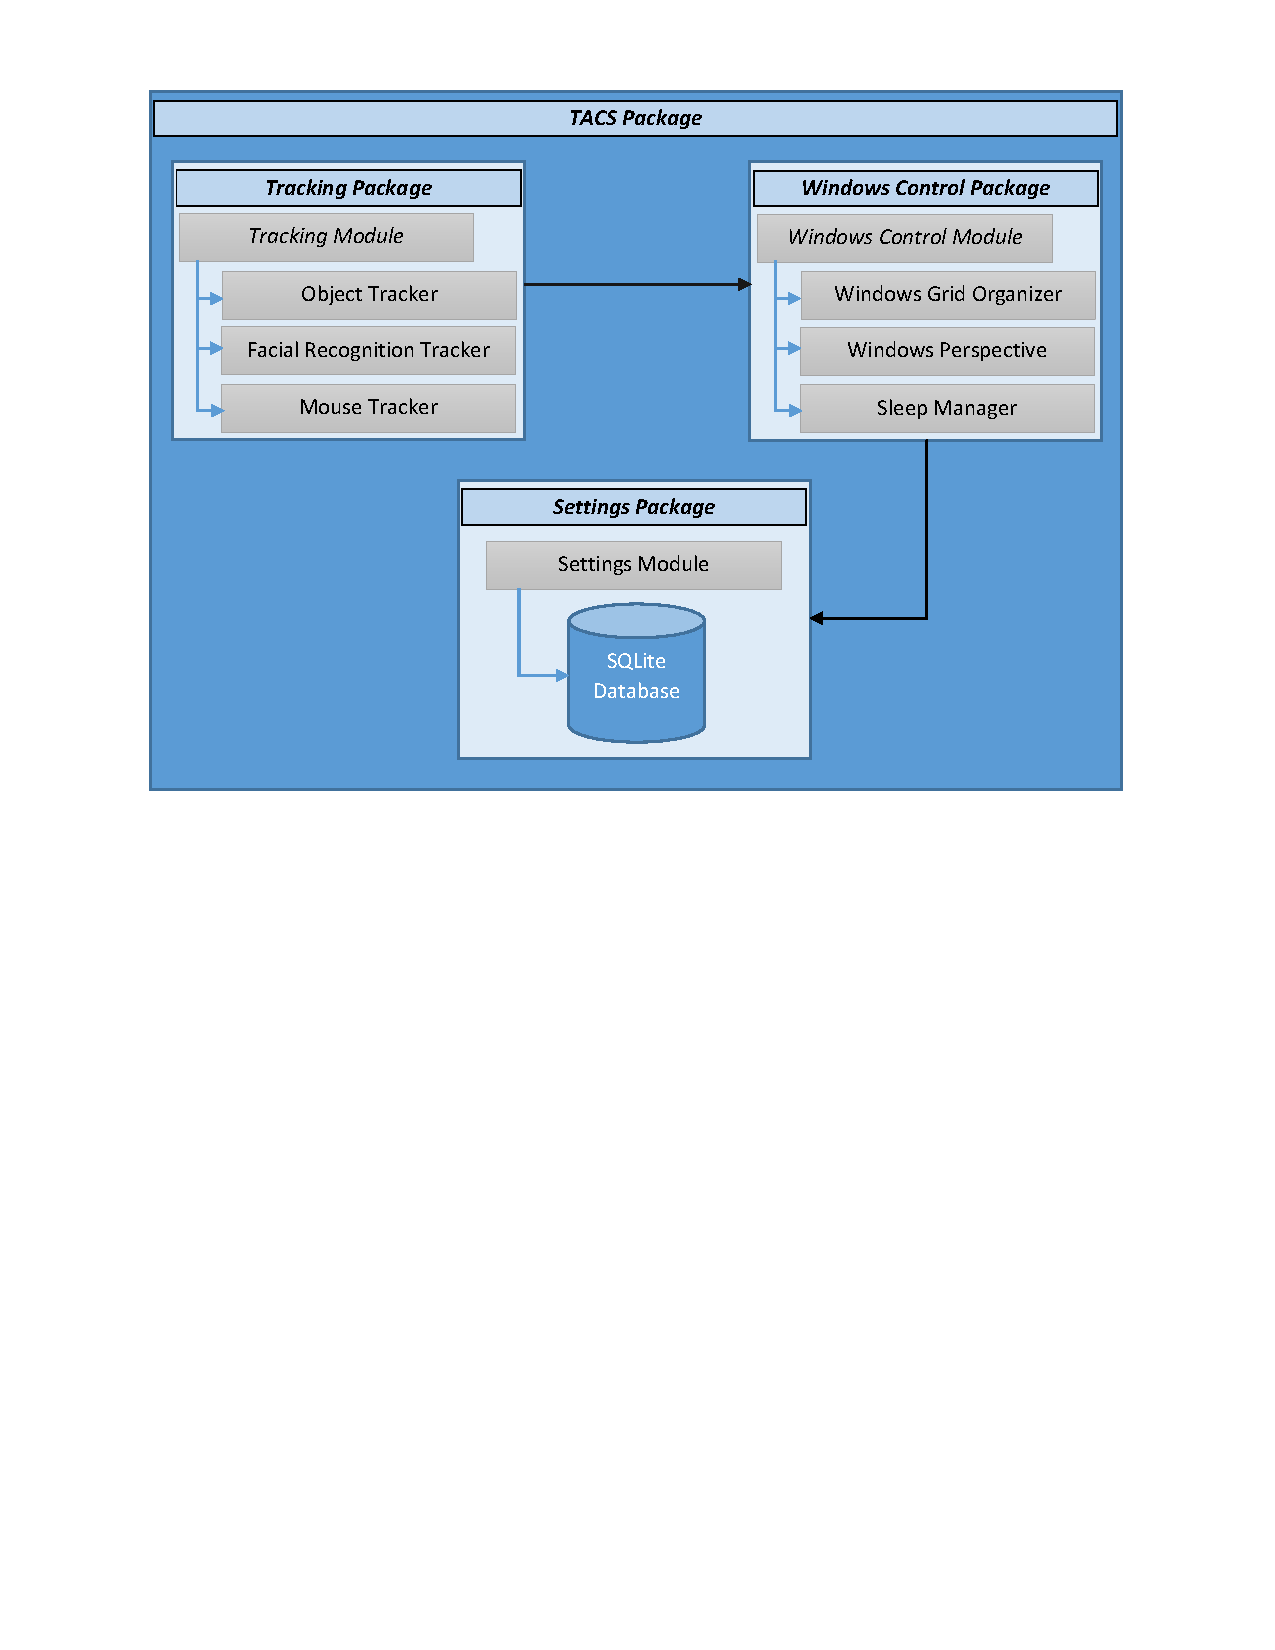
\includegraphics[trim={2cm 14cm 1cm 1cm},clip,scale=0.71]{package_diagram.pdf}
\end{center}

\newpage

\subsection{Package Definition}
\subsubsection{Tracking Package}
\begin{minipage}{\textwidth}
\begin{wrapfigure}{l}{0.45\textwidth}
  \vspace{-20pt}
  \begin{center}
	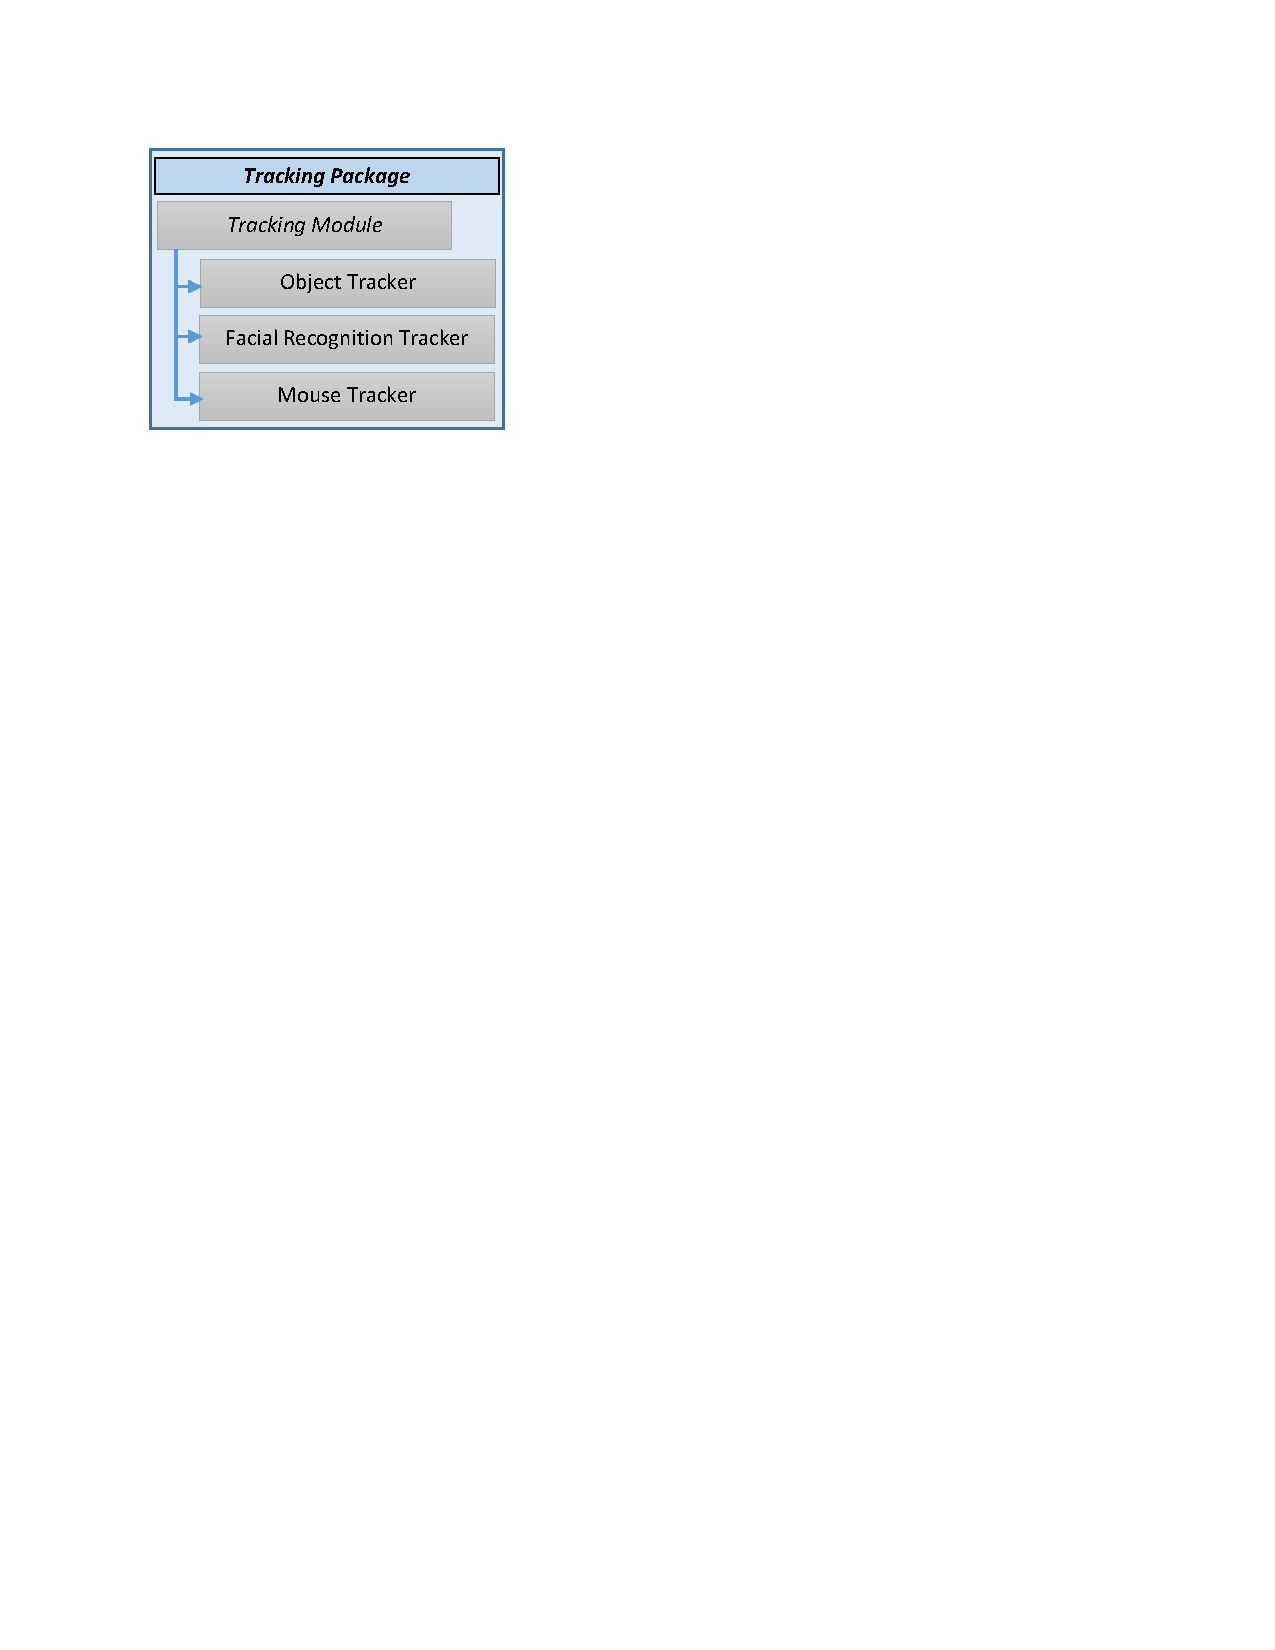
\includegraphics{tracking_package.pdf}
  \end{center}
\end{wrapfigure}
The tracking package will consist of the TrackingModule interface, and it's three sub-classes. The Tracking Module cannot be instantiated itself, only allowing the sub-class trackers to be initialized.
\end{minipage}

\vspace{+100pt}

\subsubsection{Windows Control Package}
\begin{minipage}{\textwidth}
\begin{wrapfigure}{l}{0.45\textwidth}
  \vspace{-20pt}
  \begin{center}
	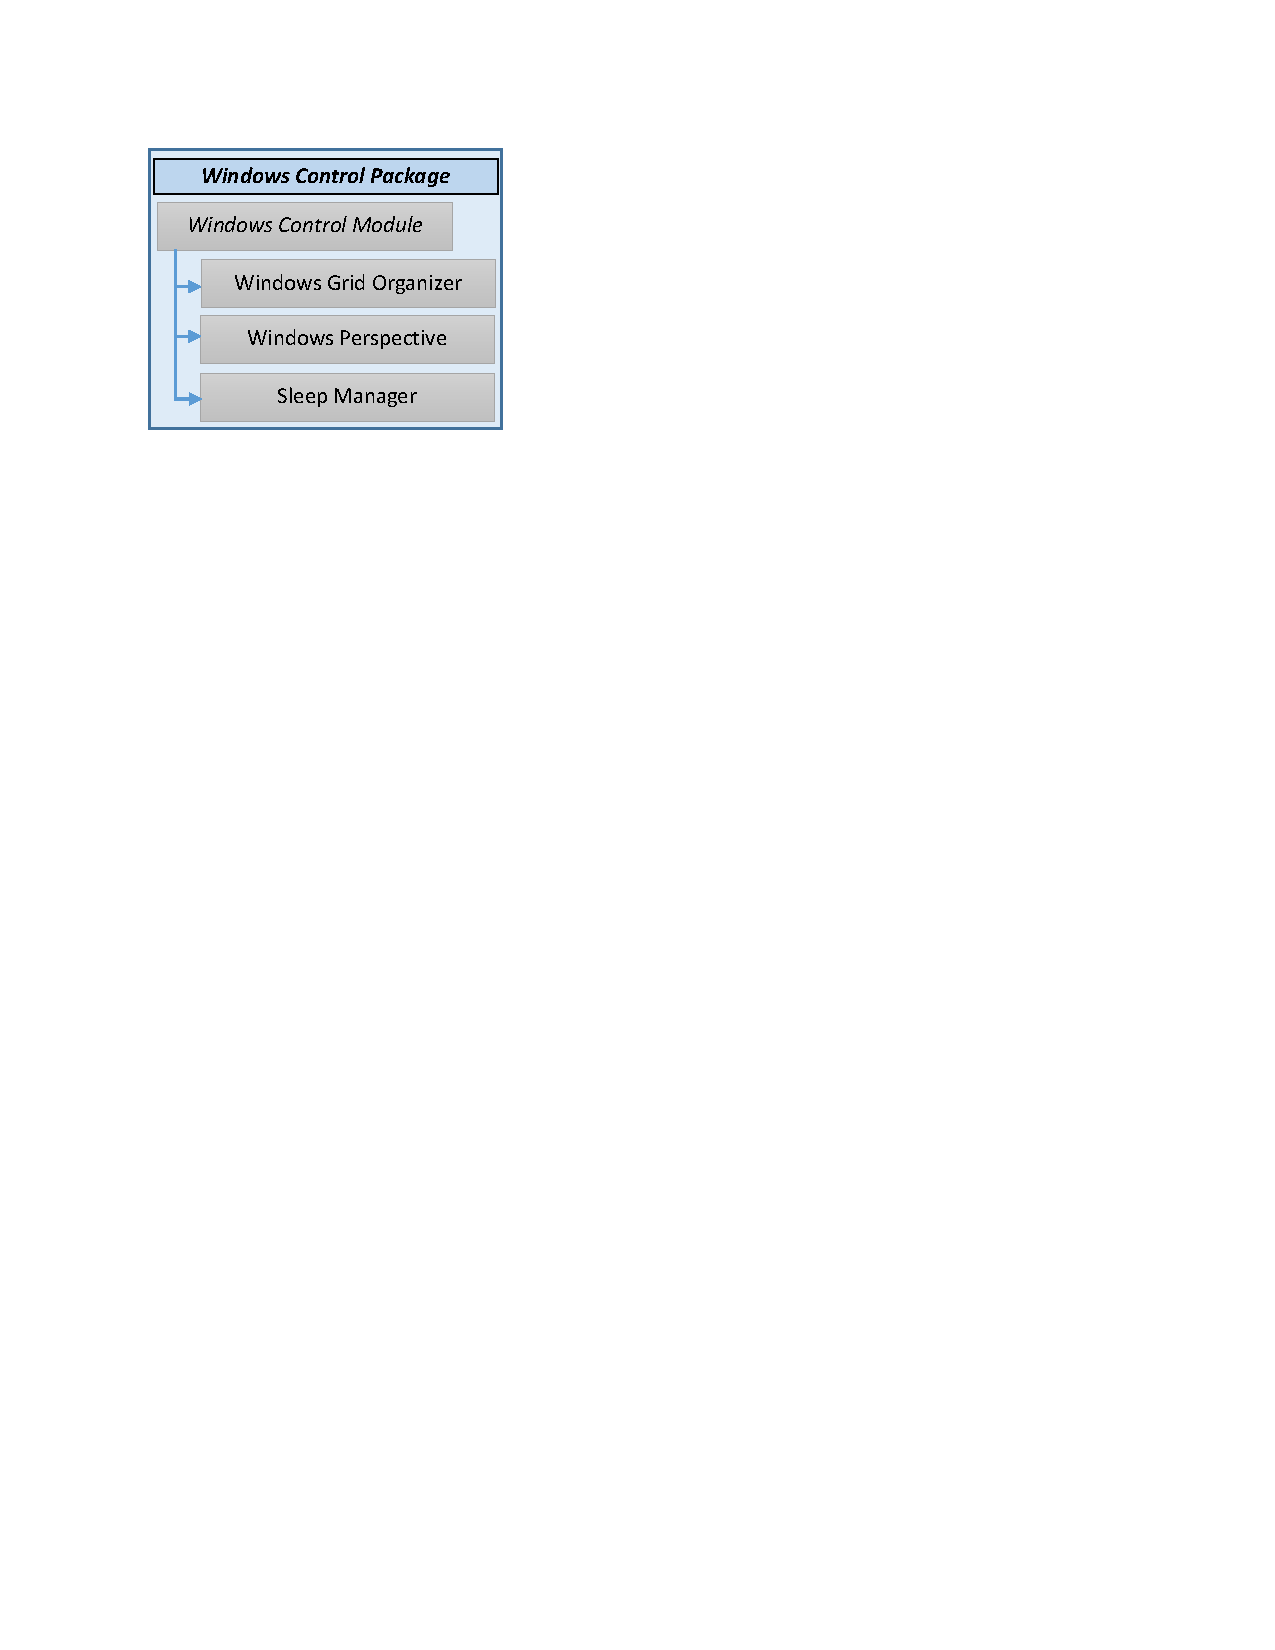
\includegraphics{windows_control_package.pdf}
  \end{center}
\end{wrapfigure}
Similarly to the tracking package, the windows control package will consist of the WindowsControlModule interface, and it's three sub-classes. The WindowsControlModule cannot be instantiated itself, only allowing the sub-class features to be initialized.
\end{minipage}

\vspace{+100pt}

\subsubsection{Settings Package}
\begin{minipage}{\textwidth}
\begin{wrapfigure}{l}{0.45\textwidth}
  \vspace{-20pt}
  \begin{center}
	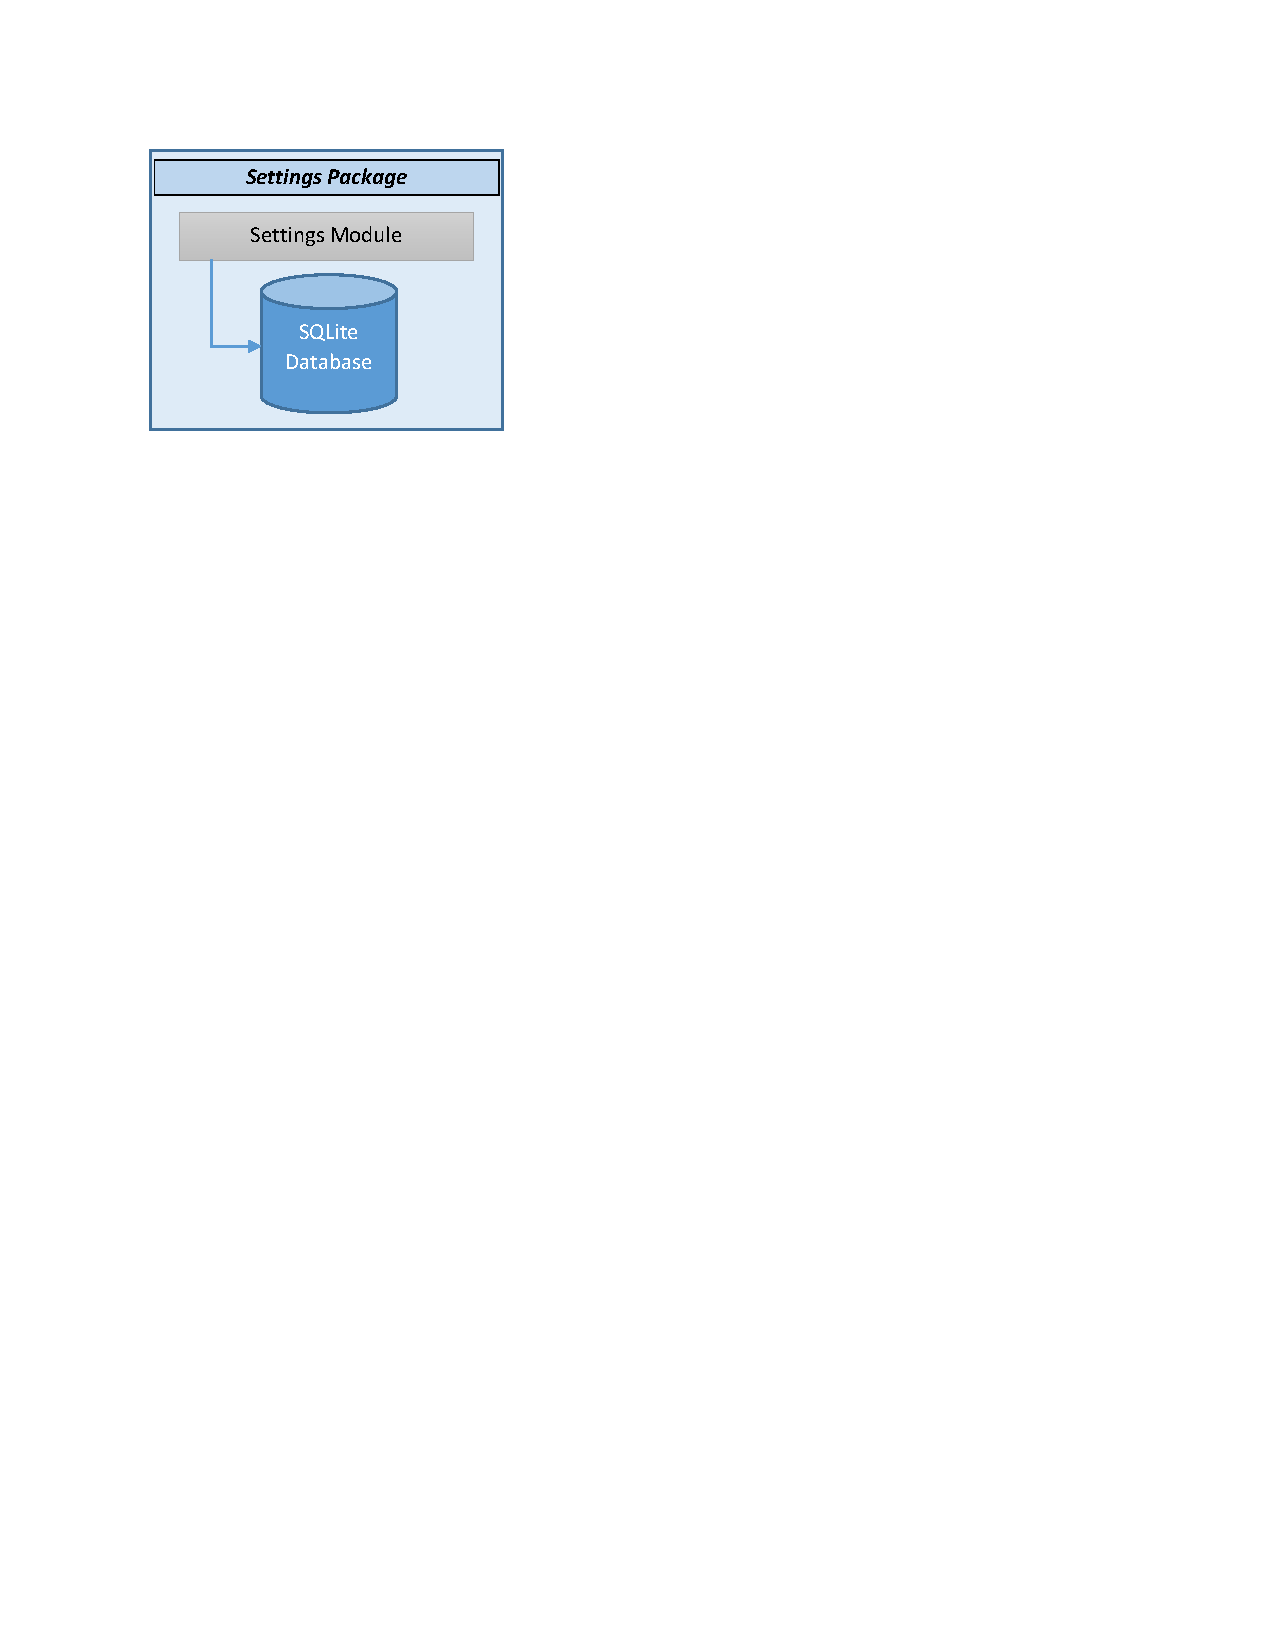
\includegraphics{settings_package.pdf}
  \end{center}
\end{wrapfigure}
The settings package will contain the SettingsModule and the local SQLite database. The SettingsModule is the only class that will write directly to the database. All other classes will pass it's information that needs to be written straight to the SettingsModule.
\end{minipage}

\section{Class Interface}
\subsection{Class Diagram}
\begin{center}
	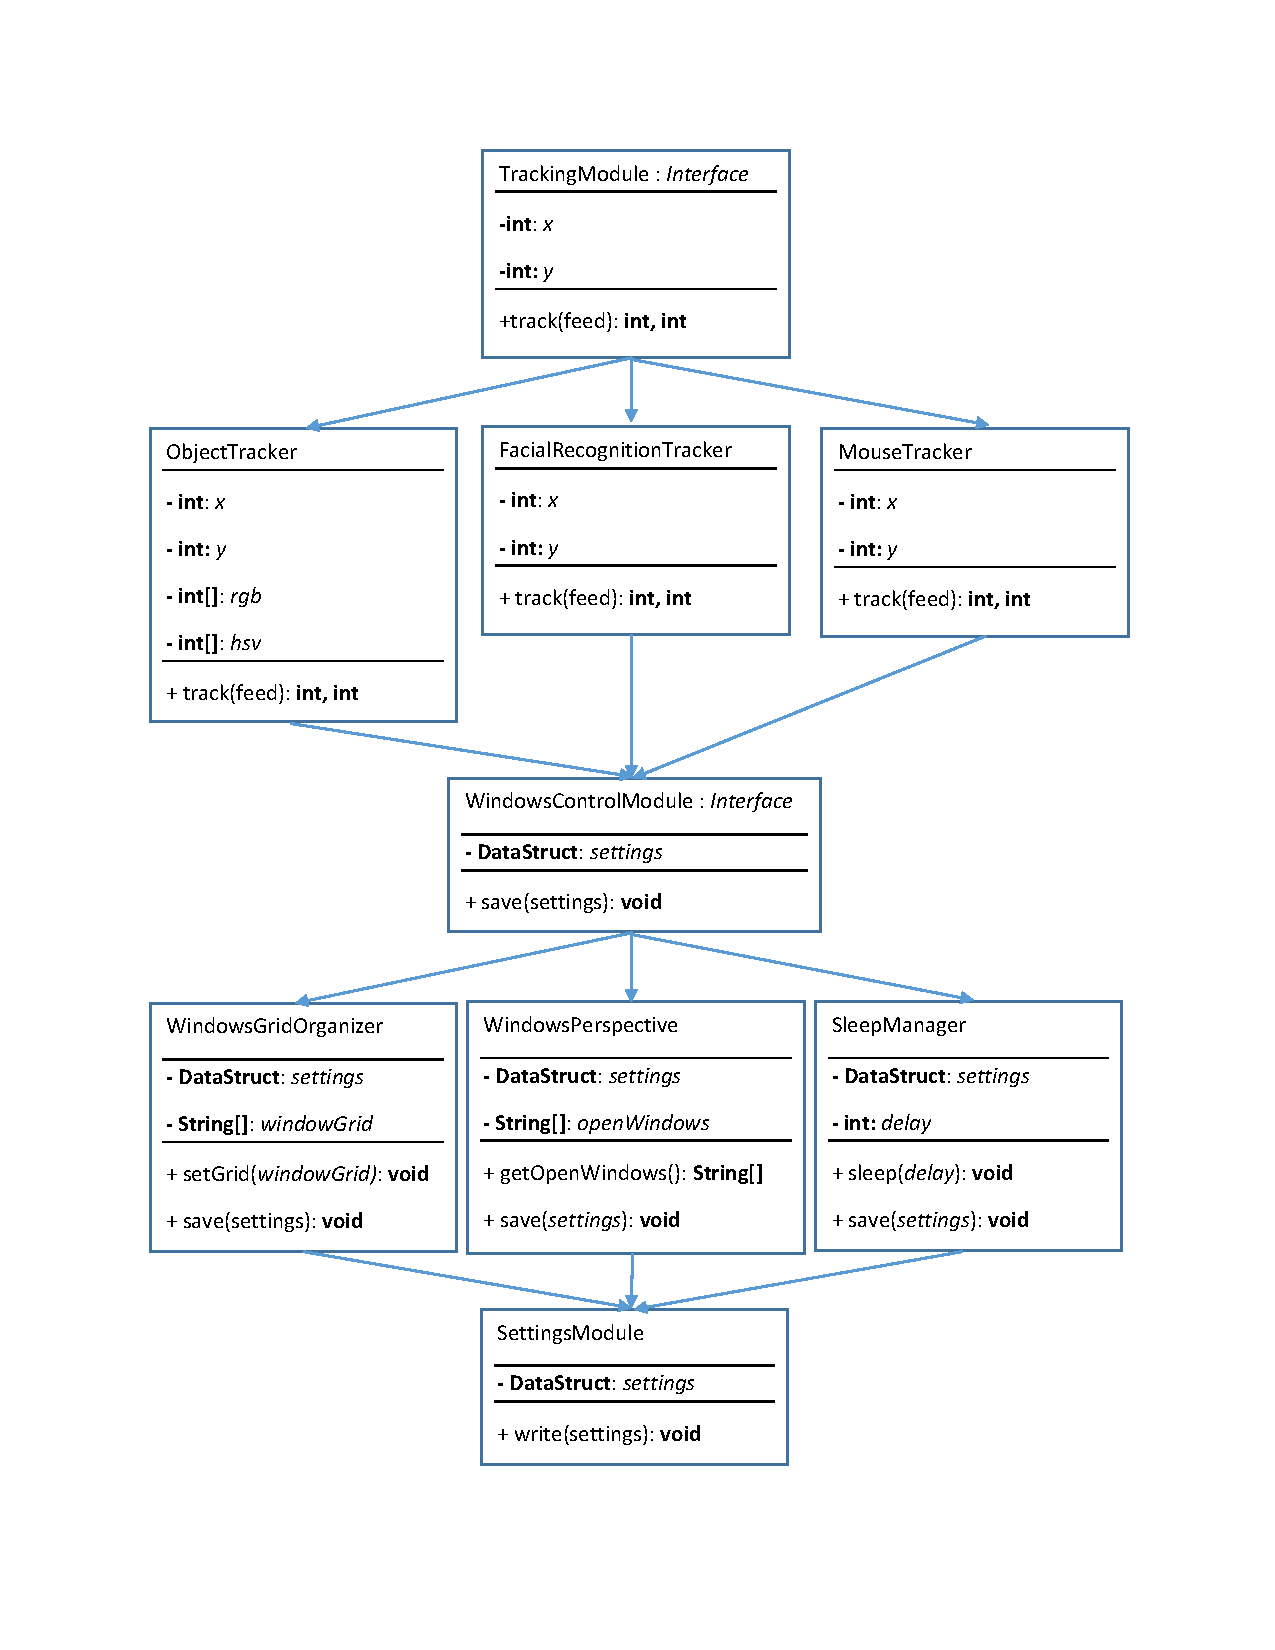
\includegraphics[width=\textwidth,height=.92\textheight,keepaspectratio]{decomposition_description.pdf}
\end{center}

\subsection{Class Definition}
\subsubsection{TrackingModule}
The TrackingModule will be an interface and super-class for the ObjectTracker, FacialRecognitionTracker, and MouseTracker. Each sub-class will hold the $x$ and $y$ values of the tracked user. The $track()$ function will be implemented differently for each sub-class. The ObjectTracker will need the RGB or the HSV values set by the user. The FRT won't need any extra variables, as it will recognize any face, not a specific face. Lastly, the MouseTracker will simply track the coordinates of the mouse and send them out as the $x$ and $y$ outputs.

\subsubsection{WindowsControlModule}
The WCM will act as a super-class for the WindowsGridOrganizer, WindowsPerspective, and SleepManager. All sub-classes will have the DataStruct, \textit{settings}, to be updated and set out as output. The WGO will keep track of which window was selected for each grid section in a String array. Then it will set the grid positioning with $setGrid()$. The WP will gather all the open windows to be resized and projected. The SleepManager will run the $sleep()$ function with the user defined delay (defaulted to a specified value). Each sub-class will output the DataStruct directly to the SettingsModule. 

\subsubsection{SettingsModule}
The SettingsModule will write the inputted DataStruct to the local SQLite database. Default values will be handled here.

\end{document}